When the numerical analysis results performed on the cb-1 via the CodeMR tool are examined, it is seen that the tool analyzes 2079 lines of code belonging to this codebase. These lines of code belong to 118 classes in 12 different packages of 4 different features which were mentioned in section \ref{section:5.3.1}. When the metric values of the analysis result performed by the CodeMR tool of the cb-1 are reviewed, some problems draw attention, although the general situation is not extremely problematic. In the figure below, a CodeMR table that reflects the general situation of cb-1 is shared. In this table, a grouped overview of the complexity, coupling and cohesion levels determined through the metric values obtained from the analysis of the codebase is shown.
\begin{figure}[ht!]
    \centering
    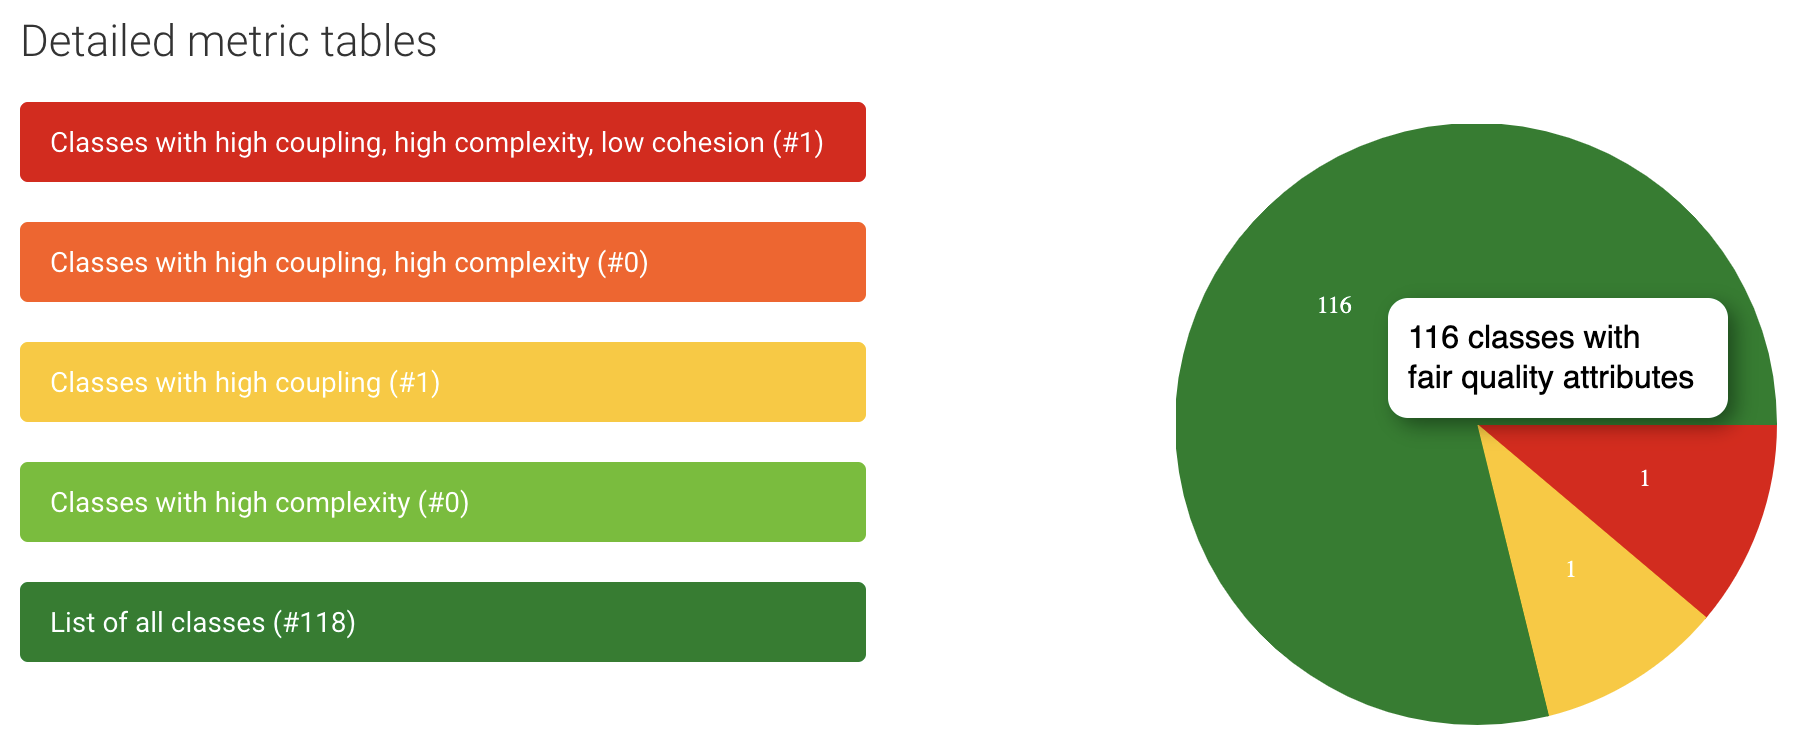
\includegraphics[scale=0.45]{figures/cb-1-metric-table.png}
    \caption{CodeMR Metrics Overview of CB-1}
    \label{fig:cb-1-metric-table.png}
\end{figure}
\FloatBarrier
The detailed evaluation of the results on the basis of metric is as follows. Among the analyzed classes, it is seen that two classes corresponding to 23\% of the total code size have medium-high WMC values. It is seen that these classes, which are classified as A and B classes, have WMC values of 61 and 58, respectively. There are also two other classes corresponding to 14\% code size have low-medium WMC values. Rest of the classes appear to have low level of WMC values.  When the values of the DIT metric of the classes are examined, it is seen that 14 classes, corresponding to 22.7\% of the total code size, have middle-upper level DIT values and the other 14 classes corresponding to 26.4\% of the total code size have low-medium level DIT values. When the NOC metric values of the classes are examined, it is seen that 7 classes corresponding to only 3.4\% of the whole codebase have low-medium NOC values and all other classes have low NOC values. According to the results, it is seen that a class, which corresponds to 12.5\% of the code volume of the application, has a very high COB value. It also appears that a class that is corresponding to 11.2\% of the application's code volume has a high COB value, and another class that is corresponding to 4.4\% of the code volume has a medium-high COB value. When the values of LCOM, the last of the selected metrics, are examined on a class basis, it is seen that 6 classes corresponding to 40.8\% of the total code size have high LCOM values. Besides, it is seen that two classes have middle-upper level LCOM values, which corresponds to approximately 4\% of the total code size. In the figure below, the results of the class-based metric values, which is detailed and interpreted above, visualized by the "Metric Distribution" method offered by the CodeMR tool are presented. Charts are in doughnut form, and information regarding the methods of creating them has been shared in the previous sections. As previously mentioned,  the size/percentage of each part in the doughnut is proportional to the size of the class/interface it represents. The detailed interpretation of the data shared in the figure below and the metric values obtained from the analysis is made in section \ref{section:6.3.1}.

\begin{figure}[ht!]
    \centering
    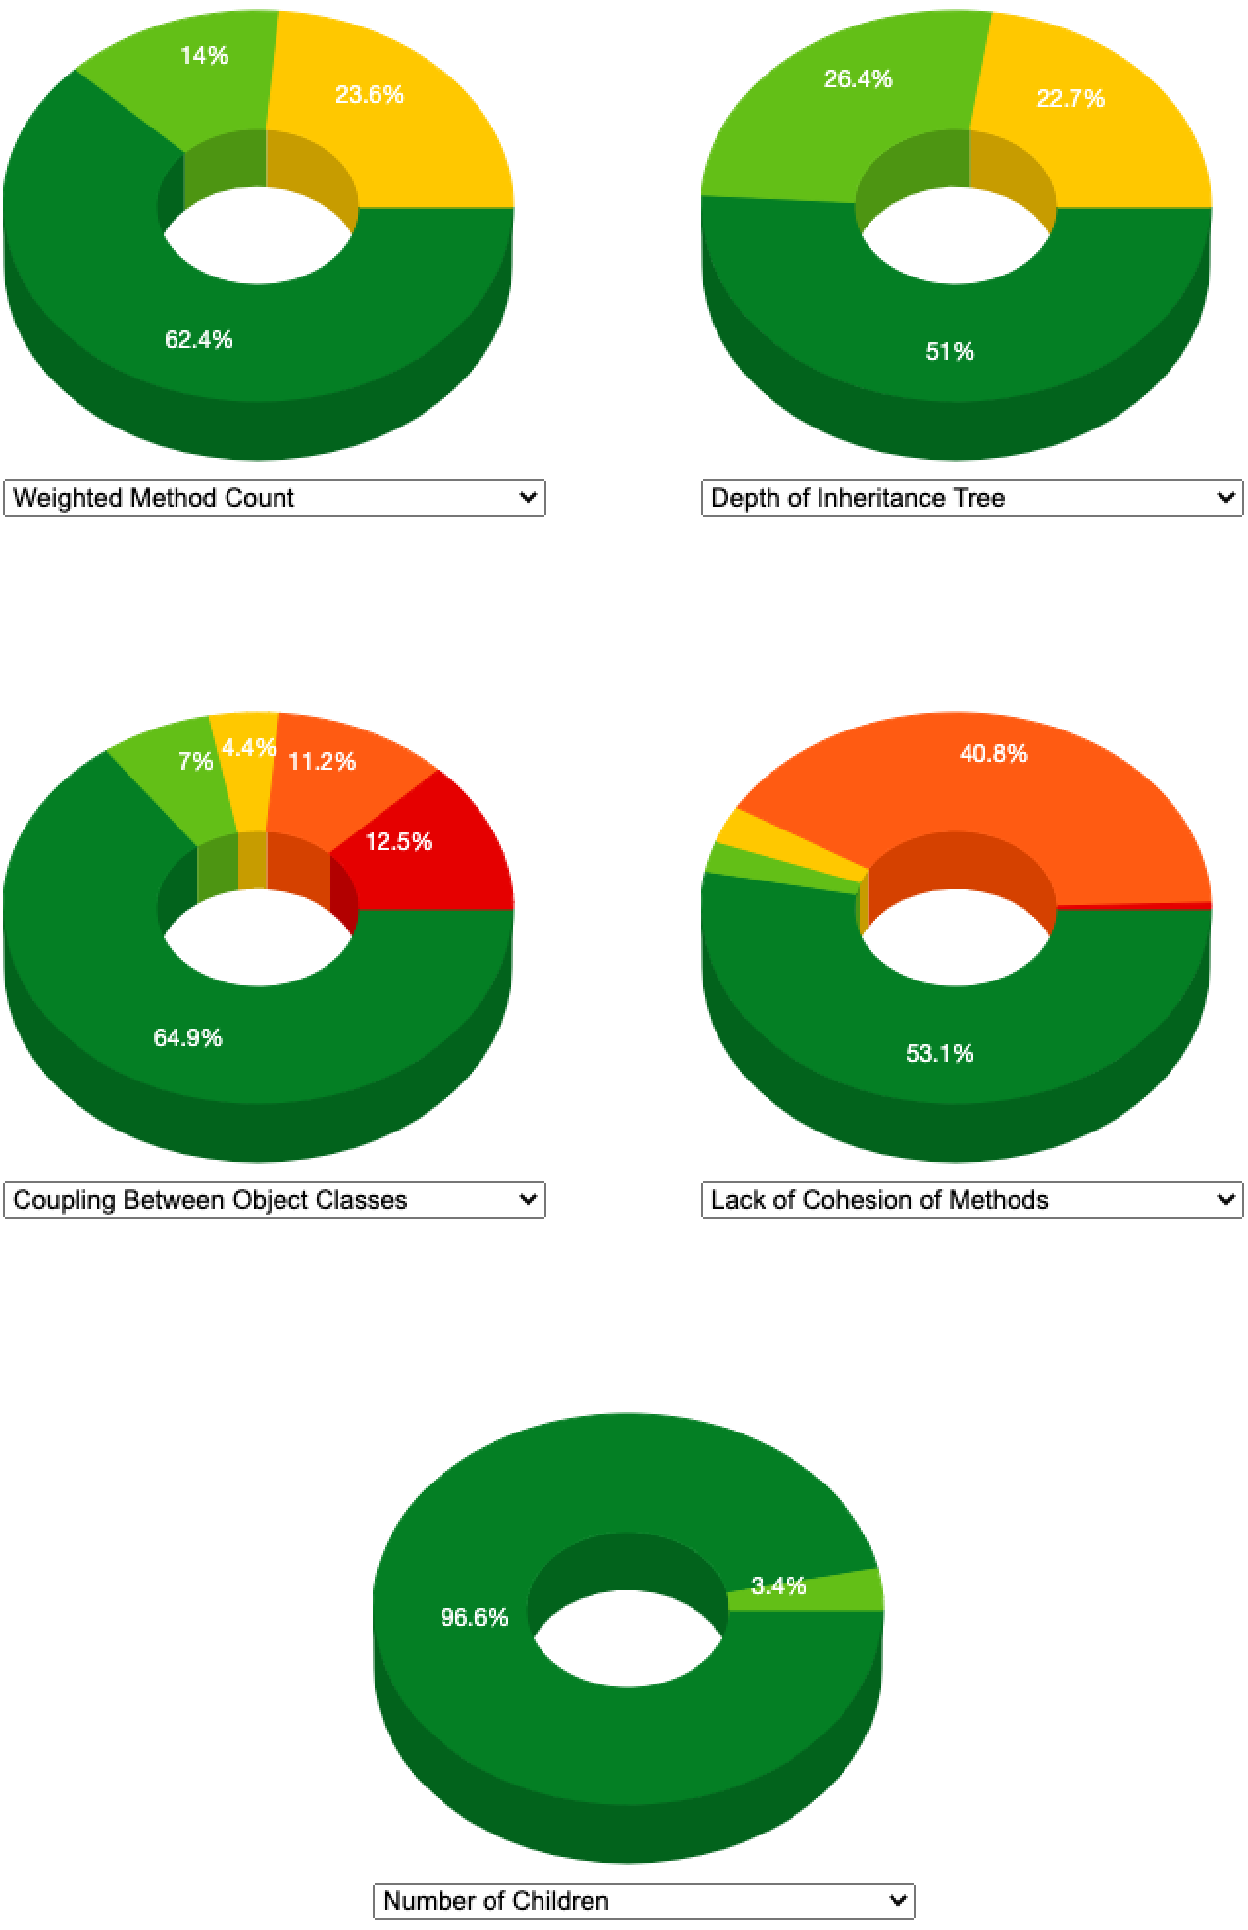
\includegraphics[scale=1]{figures/cb-1-donuts.png}
    \caption{CodeMR Metric Distribution for CB-1}
    \label{fig:cb-1-donuts}
\end{figure}
\FloatBarrier

In the figure below, a more general view of cb-1 in terms of complexity, coupling and cohesion is presented. In Fig. \ref{fig:cb-1-package}, the largest circle represents the project, while the inner circles represent the packages and the small circles inside the inner circles represent the classes. The size of each circle is directly proportional to the size of the structure it represents. The detailed interpretation of the  the figure below is made in section \ref{section:6.3.1}.

\begin{figure}[ht!]
    \centering
    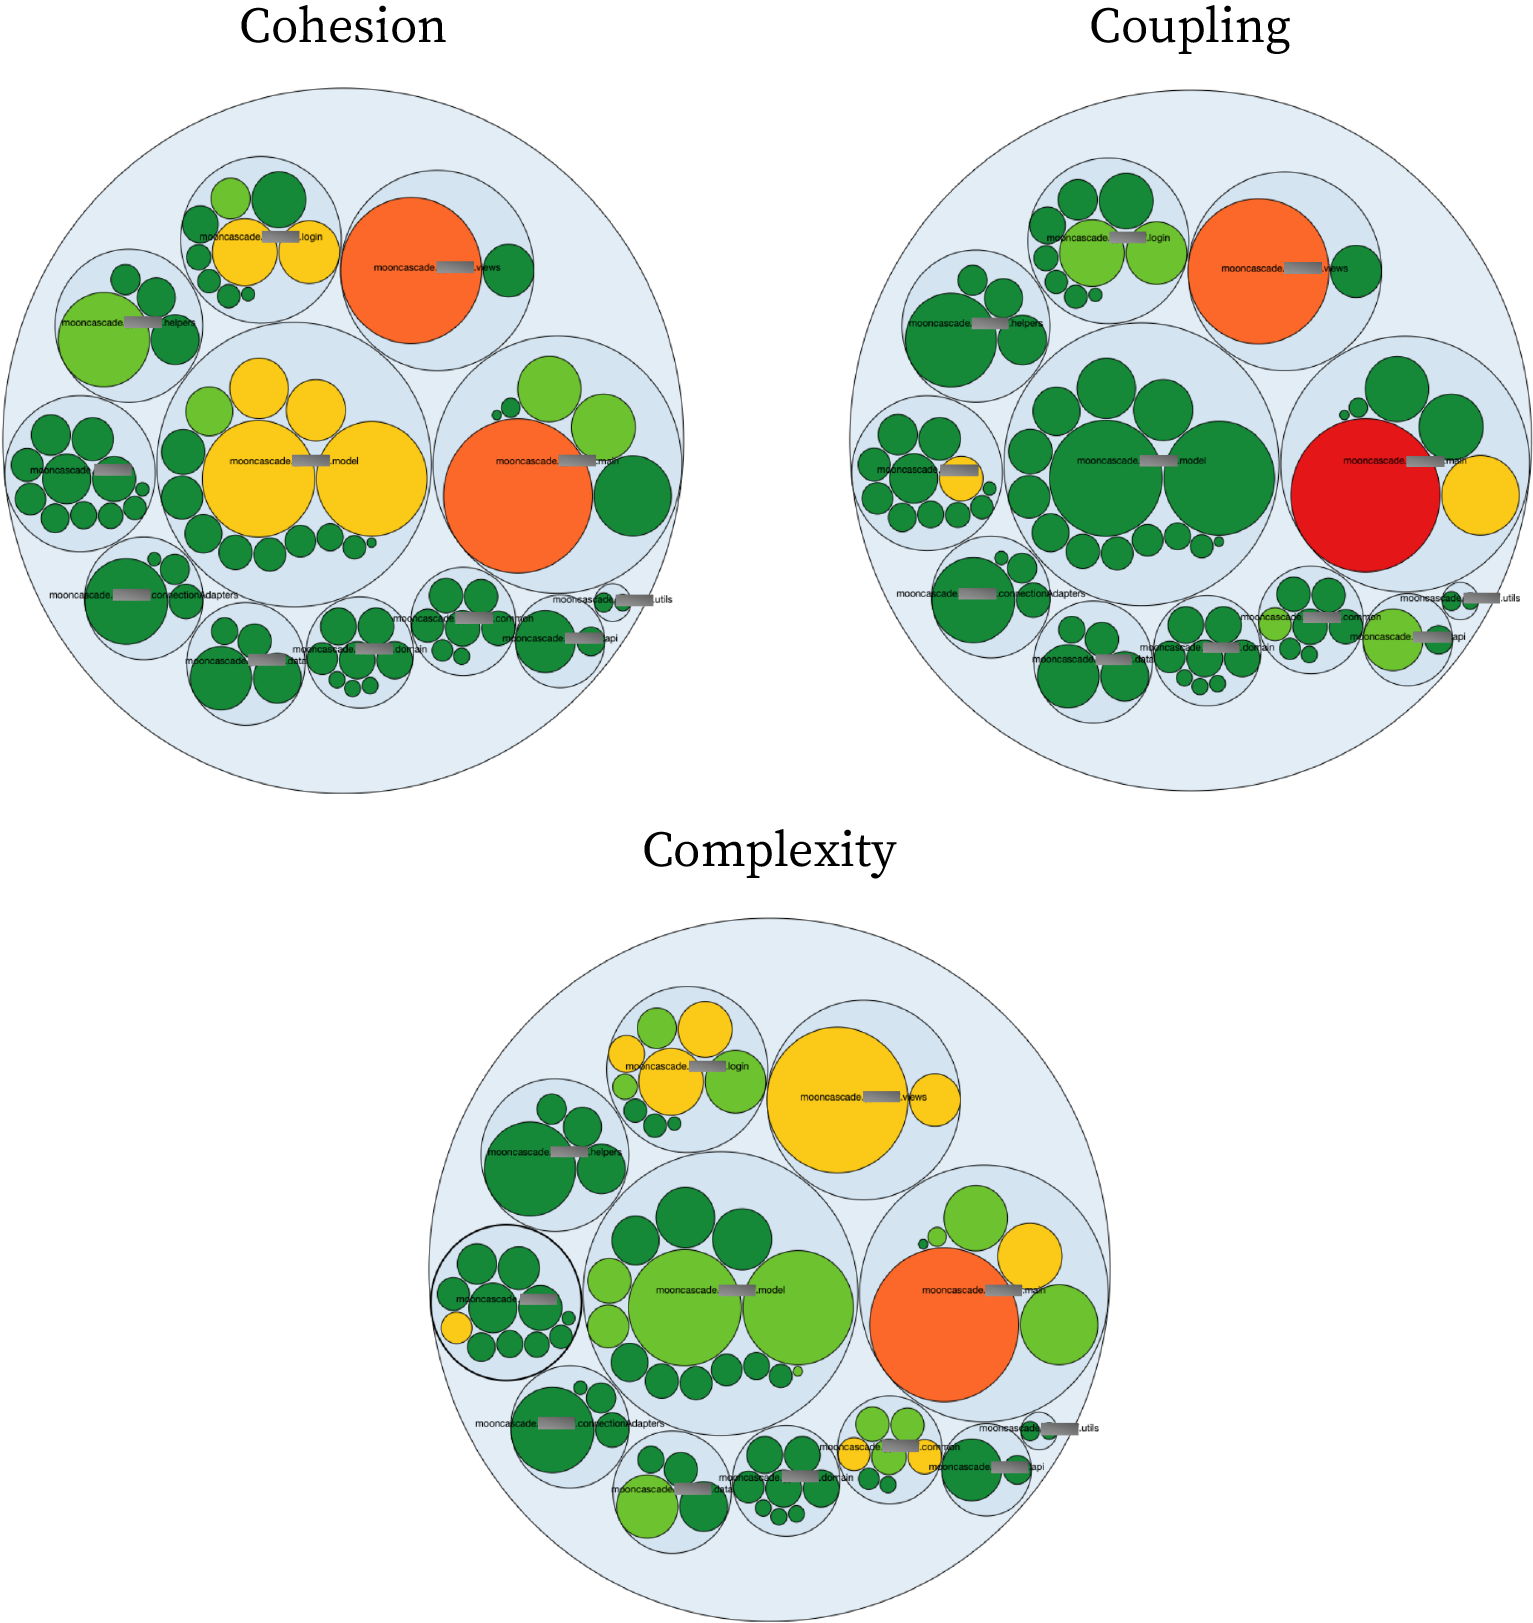
\includegraphics[scale=1.1]{figures/cb-1-package.png}
    \caption{CodeMR Metric Values by Packages for CB-1}
    \label{fig:cb-1-package}
\end{figure}
\FloatBarrier

